% \begin{table}[hptb]
%   \centering
%   \begin{tabular}{|c|c|c|c|c|}
%   \hline
%     \multicolumn{5}{|c|}{Mean Error Rate} \\
%     \hline
%     & \multicolumn{4}{c|}{Channel Model} \\
%     \hline
%     Wavelet Family & Without Channel & AWGN & Rayleigh Fading & Rician Fading\\
%     \hline
%     \multicolumn{1}{|c|}{Designed Wavelet Filters} & 1.41 x $10^{-8}$ & 0.009215 & 0.06015 & 0.000380 \\
%     \hline
%     \multicolumn{1}{|c|}{Haar} & 4.35 x $10^{-8}$ & 0.012177 & 0.06398 & 0.00411  \\
%     \hline
%     \multicolumn{1}{|c|}{Daubechies} & 2.34 x $10^{-8}$ & 0.009020 & 0.06476 & 0.000437 \\
%     \hline
%     \multicolumn{1}{|c|}{Symlets} & 2.75 x $10^{-8}$ & 0.010338 & 0.07567 & 0.000484 \\
%     \hline
%     \multicolumn{1}{|c|}{Biorthogonal} & 3.16 x $10^{-8}$ & 0.013067 & 0.06395 & 0.000411 \\
%     \hline
%   \end{tabular}
% \end{table}

% \begin{table}[hptb]
%   \centering
%   \begin{tabular}{|c|c|c|c|c|}
%   \hline
%     \multicolumn{3}{|c|}{Mean Error Rate} \\
%     \hline
%     & \multicolumn{2}{c|}{Channel Model} \\
%     \hline
%     Wavelet Family & Without Channel & AWGN \\
%     \hline
%     \multicolumn{1}{|c|}{Designed Wavelet Filters} & 1.41 x $10^{-8}$ & 0.009215  \\
%     \hline
%     \multicolumn{1}{|c|}{Haar} & 4.35 x $10^{-8}$ & 0.012177   \\
%     \hline
%     \multicolumn{1}{|c|}{Daubechies} & 2.34 x $10^{-8}$ & 0.009020 \\
%     \hline
%     \multicolumn{1}{|c|}{Symlets} & 2.75 x $10^{-8}$ & 0.010338  \\
%     \hline
%     \multicolumn{1}{|c|}{Biorthogonal} & 3.16 x $10^{-8}$ & 0.013067 \\
%     \hline
%   \end{tabular}
% \caption{\label{tab:sim}Mean Error Rate of the System for SNR = $-20$ dBW}
% \end{table}

% \begin{table}[htpb]
%     \centering
%     \begin{tabular}{|c|c|c|}
%     \hline
%     \multicolumn{3}{|c|}{Mean Error Rate} \\
%     \hline
%     & \multicolumn{2}{c|}{Channel Model} \\
%     \hline
%       Average Path Gain (dBW)  & Rayleigh Fading & Rician Fading\\
%       \hline
%      \multicolumn{1}{|c|}{-100} & &  \\
%          \hline
%       \multicolumn{1}{|c|}{-50}  & 0.06015 & 0.000380 \\
%          \hline
%       \multicolumn{1}{|c|}{-20}  &  &  \\
%          \hline
%       \multicolumn{1}{|c|}{-5}   & & \\ 
%          \hline 
%       \multicolumn{1}{|c|}{10}   & 0.000019 &\\ 
%          \hline
%       \multicolumn{1}{|c|}{30}   &  &\\
%          \hline 
%       \multicolumn{1}{|c|}{50}  &  &\\
%          \hline
%     \end{tabular}
%     \caption{Mean Error Rate of the System for Multipath Fading Channels.}
%     \label{tab:error_fading}
% \end{table}


% \begin{figure}[htpb]
% \centering
% \begin{tabular}{cc}
%   \includegraphics[width=75mm]{H0_pzmap.jpg} & \includegraphics[width=75mm]{G0_pzmap.jpg} \\
% (a) Synthesis filter $H_0$ & (b) Analysis filter $G_0$ \\[8pt]
%  \includegraphics[width=75mm]{H1_pzmap.jpg} & \includegraphics[width=75mm]{G1_pzmap.jpg} \\
% (c) Synthesis filter $H_1$  & (d) Analysis filter $G_1$  \\ [8pt]
% \includegraphics[width=75mm]{H2_pzmap.jpg} & \includegraphics[width=75mm]{G2_pzmap.jpg} \\
% (e) Synthesis filter $H_2$ & (f) Analysis filter $G_2$\\[8pt]
% \end{tabular}
% \caption{Pole-Zero plots of the designed filters.}
% \label{pzmap}
% \end{figure}

% \vspace{1cm}
% \begin{figure}[htpb]
% \centering
% \begin{tabular}{cc}
% 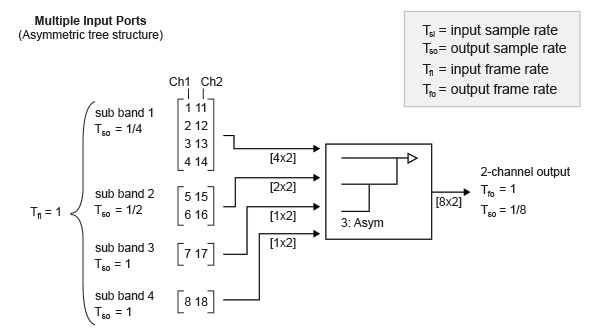
\includegraphics[width=77mm]{dyadic_synth_diagram.jpg} & 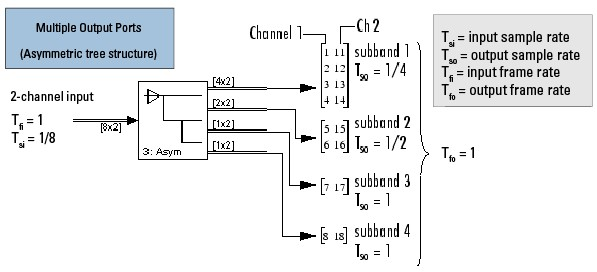
\includegraphics[ width=77mm]{dyadic_analysis_diagram.jpg} \\
% (a) DWT Synthesis Filter Bank & (b) DWT Analysis Filter Bank \\[6pt]
% \end{tabular}
% \caption{Block Diagram of DWT Analysis and Synthesis Filter Bank Objects.}
% \label{dyadic}
% \end{figure}

% \[
% \begin{bmatrix} \hat{x}_1
% \\ \hat{x}_2
% \\ \hat{x}_3
% \end{bmatrix}
% =                 
% \begin{bmatrix}
% G_0(z)  & G_1(z) & G_2(z) \\ 
% G_0(-z) & G_1(-z) & G_2(-z)\\ 
% G_0(z) \hspace{1mm} z^{1/4} & G_1(z) \hspace{1mm} z^{1/4} & G_2(z) \hspace{1mm}z^{1/4} 
% \end{bmatrix}
         
% \begin{bmatrix}
% H_0(z)  & H_1(z) & H_2(z) \\ 
% H_0(-z) & H_1(-z) & H_2(-z)\\ 
% H_0(z) \hspace{1mm} z^{-1/4} & H_1(z) \hspace{1mm} z^{-1/4} & H_2(z) \hspace{1mm}z^{-1/4} 
% \end{bmatrix}

% \begin{bmatrix} x_1(z^4)
% \\ x_2(z^4)
% \\ x_3(z^4)

% \end{bmatrix}
% \]

% \begin{figure}[htpb]
% \centering
% 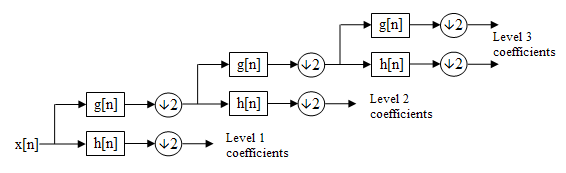
\includegraphics[width=3.5in]{Wavelets_-_Filter_Bank.png}
% \caption{Block diagram of Discrete Wavelet Transform.}
% \label{dwt}
% \end{figure}

% \section{Motivation}
% This work was motivated by the need to emulate the loads which allows the user to test both the hardware and the software of the inverter. The virtual load can provide different load characteristics with which the control algorithms and inverter design can be
% tested. The flexibility of the load emulation allows the designer of the control algorithms to experiment with different designs safe in the knowledge that if something goes wrong expensive damage to the inverter and machine will not result. A rotating machine cannot be stopped instantly: it has inertia. The load emulation contains no rotating parts, it is made up of fast acting power electronics which can handle a fault situation and prevent unnecessary damage.\par
% The load emulation system has regeneration capability, as the power flow from the inverter can be returned to the mains supply. When testing an inverter with an actual machine, the machine uses this power for rotation and it is therefore lost. As well as being a small energy benefit this also reduces the laboratory power supply requirements.


% Chapter 5: Survey on current control methods are presented in this chapter. Investigation on the basic performance of current controller will be made using circuit simulation software SEQUEL. The results obtained from simulation are discussed.\\
% Chapter 6: Some of the important design issues will be highlighted in this chapter. Being a non-ideal device, the inverter has many drawbacks. Dead-time between the IGBT switching, resistive voltage drop of the switching components and the DC-link voltage fluctuations have been identified as the most problematic non-idealizes. Analysis of the adverse effects of these problems and compensation methods will be the focus of this chapter.\\
% Chapter 7:  The problem of ripple output at the inverter legs and bidirectional power flow  will be the focus of this chapter.\\
% Chapter 8: Conclusions and discussion on future course of research work.\\